\documentclass[11pt, aspectratio=169, table]{beamer}



\usepackage[utf8]{inputenc}
\usepackage{amsmath}
\renewcommand{\footnotesize}{\scriptsize}
\setbeamertemplate{footline}[frame number]
\usepackage{ulem}
\usepackage{programs}

\usepackage{multirow}
\usepackage{tabularx}

\usepackage{fretish}

\usepackage{appendixnumberbeamer}

\setbeamertemplate{background canvas}[bottom=white!10,top=white!10]

\usefonttheme[onlysmall]{structurebold}
%\useinnertheme{rounded}
\setbeamertemplate{itemize items}[triangle]


%%%tikzstuff
\usepackage{tikz}
\usetikzlibrary{shapes.geometric, arrows}
\tikzstyle{fragment} = [rectangle, minimum width=2em, minimum height=2em, text centered, draw=black, fill={rgb:black,1;white,3}]
\tikzstyle{req} = [rectangle, minimum width=2em, minimum height=2em, text centered, draw=black]
\tikzstyle{arrow} = [thick,->,>=stealth]


\usetheme{Madrid}
%\usetheme{Rochester}%
%\usetheme{JuanLesPins}%
%\usecolortheme{beaver}
%\usecolortheme{whale}%



\pdfpageattr {/Group << /S /Transparency /I true /CS /DeviceRGB>>}

%Corporate Brand of University 
\definecolor{UniBlue}{RGB}{0,55,113}
\definecolor{UniYellow}{RGB}{240,171,0}
\definecolor{UniRed}{RGB}{130,35,39}
\definecolor{UniGreen}{RGB}{0,103,120}

% set enumerations to squares, since balls look horrible in gold
\setbeamertemplate{enumerate item}[square]{}

% set color scheme to uni colours
\setbeamercolor{palette primary}{fg=UniYellow, bg=UniGreen}
\setbeamercolor{palette secondary}{fg=white, bg=UniBlue}
\setbeamercolor{palette tertiary}{fg=white, bg=UniRed}
\setbeamercolor{palette quaternary}{fg=white, bg=UniRed}

\setbeamercolor{structure}{fg=UniGreen}
% remove this if you want UniBlue items (or overwrite for something funky) 
\setbeamercolor{item}{fg=UniRed}

% the following lines overwrite the normal example and alert block colors
% even though these are "official" university brand colours, I am not a big
% fan of them... use them at your own discretion
% set color of alert
\setbeamercolor{block title alerted}{bg=UniRed!80!black}
% set color of example
\setbeamercolor{block title example}{bg=UniGreen!85!black}


\setbeamercolor{footbox1}{fg=UniYellow,bg=UniBlue}
\setbeamercolor{footbox2}{fg=UniYellow,bg=UniGreen}


%\setbeamertemplate{footline}[frame number]
\setbeamertemplate{footline}
{%
\begin{beamercolorbox}[wd=0.2\textwidth,ht=3ex,dp=1.5ex,leftskip=.5em,rightskip=.5em]{footbox1}%
\usebeamerfont{author in head/foot}%
\hspace{1em}\insertshortauthor%
\end{beamercolorbox}%
\vspace*{-4.5ex}\hspace*{0.2\textwidth}%
\begin{beamercolorbox}[wd=0.6\textwidth,ht=3ex,dp=1.5ex,center,leftskip=.5em]{footbox2}%
\usebeamerfont{title in head/foot}%
\centering
\insertshorttitle%
\end{beamercolorbox}%
\begin{beamercolorbox}[wd=0.2\textwidth,ht=3ex,dp=1.5ex,right,leftskip=.5em]{footbox1}%

\hfill\insertframenumber/\inserttotalframenumber\hspace{1em}
\end{beamercolorbox}

}

\setbeamertemplate{caption}[numbered]
\setbeamertemplate{itemize items}[triangle]



\setbeamertemplate{caption}[numbered]

\title[Sharper Specs for Smarter Drones]{Sharper Specs for Smarter Drones: \\Formalising Requirements with FRET} 

\date{10$^{th}$ of April 2025}

\author[]{\emph{Ois\'{i}n Sheridan} \and Leandro Buss Becker \and Marie Farrell \and Matt Luckcuck \and Rosemary Monahan}
\institute[]{
Department of Computer Science, Maynooth University/Hamilton Institute, Maynooth, Ireland
\and
Automation and Systems Department, Federal University of Santa Catarina, Florian\'{o}polis, Brazil
\and
Department of Computer Science, The University of Manchester, Manchester, UK
\and
School of Computer Science, University of Nottingham, Nottingham, UK
}


%% This adds a section heading slide is you use \section{}
\AtBeginSection[]{
  \begin{frame}
  \vfill
  \centering
  \begin{beamercolorbox}[sep=8pt,center,shadow=true,rounded=true]{title}
    \usebeamerfont{title}\insertsectionhead\par%
  \end{beamercolorbox}
  \vfill
  \end{frame}
}


%This removes the navigation symbols from the bottom of the slides
\setbeamertemplate{navigation symbols}{}


\begin{document}

%
\begin{frame}

\begin{minipage}{0.25\textwidth}
\begin{flushleft}

\includegraphics[height=4em]{images/mu-logo.png}
\end{flushleft}
\end{minipage}\noindent
\begin{minipage}{0.2\textwidth}
\centering

\includegraphics[height=4em]{images/UFSC-logo.png}
\end{minipage}\noindent
\begin{minipage}{0.27\textwidth}
\begin{flushright}

\includegraphics[height=4em]{images/manchester-logo.png}
\end{flushright}
\end{minipage}\noindent
\begin{minipage}{0.3\textwidth}
\begin{flushright}

\includegraphics[height=4em]{images/nottingham-logo.png}
\end{flushright}
\end{minipage}\noindent

\titlepage

\end{frame}



\begin{frame}{Introduction}

\begin{block}{Overview}

\begin{itemize}
    \item We describe the process of formalising the natural-language requirements for a tilt-rotor drone using the Formal Requirements Elicitation Tool (FRET).

    \item This requirements set evolved over four distinct versions as new information was elicited and incorporated into the FRETish specification.

    \item Our two concrete outputs are the formalised requirement set, which we will use in our ongoing development and verification of ProVANT; and metrics about the requirements.
    
    \item We present guidance for  requirements elicitation and formalisation with FRET.  
We highlight situations where it was difficult to formalise these requirements and describe potential improvements to FRET to address these difficulties.
	
\end{itemize}
\end{block}
\end{frame}

\section{Case Study -- ProVANT Emergentia Tilt-Rotor Drone}

\begin{frame}{Case Study -- Tilt-Rotor Drone}
\centering
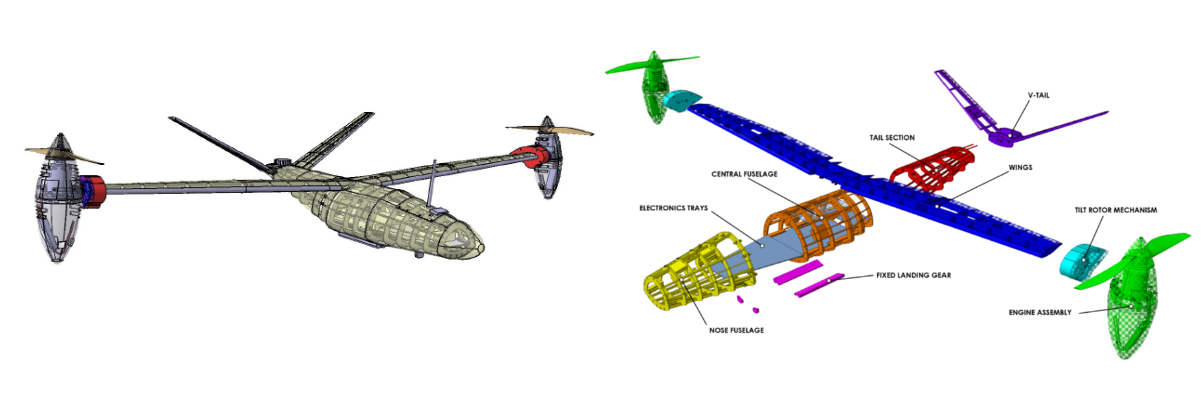
\includegraphics[width=\textwidth]{images/drone-overview.png}
\vspace{-8mm}
\begin{block}{}
	\begin{itemize}
		\item At the latter stage of development under the ProVANT Emergantia project
		
		\item The project is a collaboration among two Brazilian universities, Federal University of Minas Gerais (UFMG) and Federal University of Santa Catarina (UFSC), along with the University of Seville, Spain.
	\end{itemize}
\end{block}
\end{frame}

\begin{frame}{Case Study -- Tilt-Rotor Drone}
\begin{block}{}
	\begin{itemize}
		\item The drone can perform hovering and Vertical Take-off and Landing (VTOL) manoeuvres, as well as cruise flight as a fixed-wing aircraft.
		
		\item The architecture for the Drone's computing system comprises four main components:
		\begin{itemize}
		\item Raspberry Pi: Gathers sensor data and communicates with the Ground Control Station.
			\item Jetson: Processes sensor data and runs the control algorithm.
			\item Nucleos: the active nucleo interfaces with the drone's actuators and some sensors. Can also run a backup control algorithm in the case of a failure. There are two nucleos for reliability.
		\end{itemize}
		
		\item The set of requirements for the ProVANT Emergentia drone includes aspects related to:
		\begin{enumerate}
			\item operation features present during simulations and during real executions
			\item remote monitoring configurations
			\item timing constraints associated with the control loop
			\item operation modes under failure conditions
		\end{enumerate}
	\end{itemize}
\end{block}
\end{frame}

\section{Formalisation with FRET}

\begin{frame}{The Formal Requirements Elicitation Tool (FRET)}
\centering
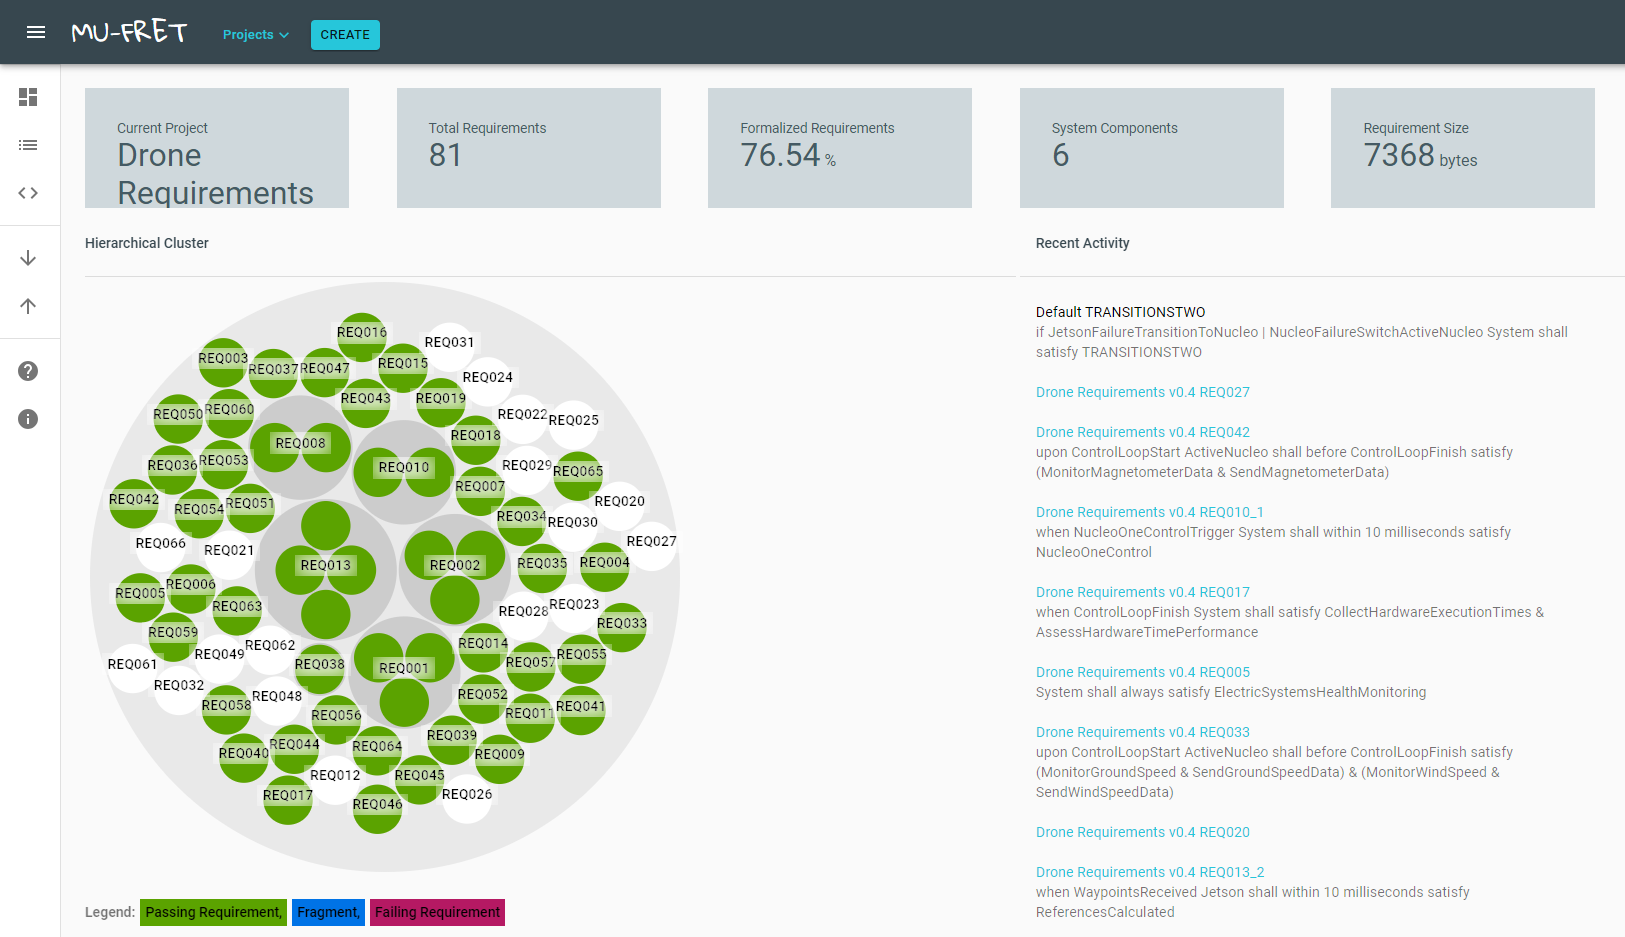
\includegraphics[width=0.8\textwidth]{images/mu-fret-dashboard.png}
\end{frame}


\begin{frame}{The Formal Requirements Elicitation Tool (FRET)}
\begin{minipage}{0.55\textwidth}
	\begin{block}{FRET}
		\begin{itemize}
			\item An open source tool for requirements engineering developed by NASA
			
			\item Requirements are written in a structured natural-language called FRETish
			
			\item FRET provides automated translations from FRETish to CoCoSpec contracts, which can be verified with the Kind2 model checker, and Copilot runtime monitors

                \item Formalised requirements are indicated in green, while those in white have not been formalised

		\end{itemize}
	\end{block}
\end{minipage}\noindent
\begin{minipage}{0.43\textwidth}
	\centering
	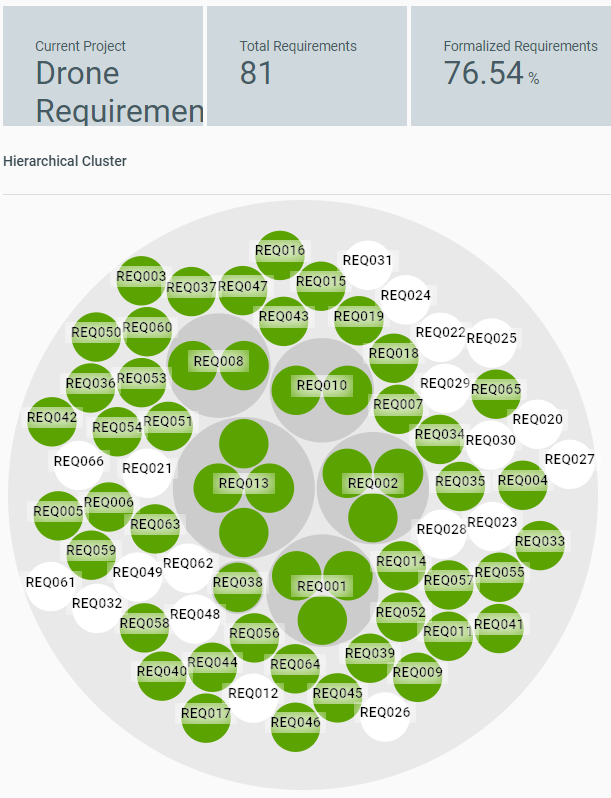
\includegraphics[width=0.86\textwidth]{images/drone-reqs-circle-diagram-no-legend.png}
\end{minipage}
\end{frame}


\begin{frame}
\centering
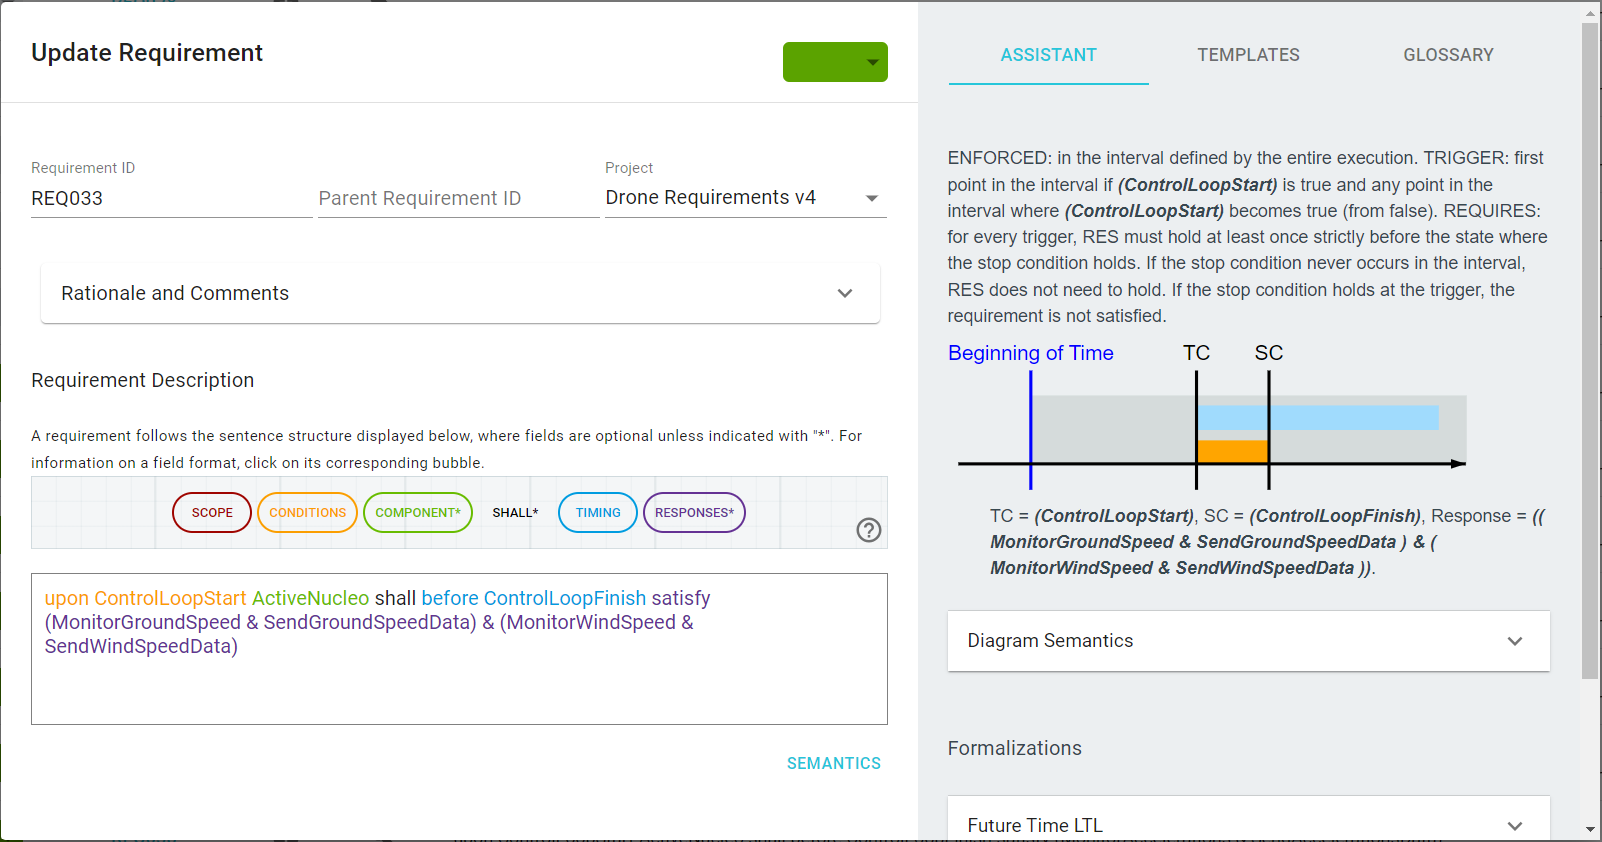
\includegraphics[width=\textwidth]{images/Drone-REQ033.png}
\end{frame}



\end{document}
